\chapter{Introduction}


%Verifikation ist wichtig
%
%Arrays sind schwierig
%
%Es gibt das von Cousot


Dividing any scalar value by zero is undefined behaviour in most programming languages and will certainly throw an error. When an experienced programmer is writing code, they make sure to include checks to rule out this behaviour. But when code becomes more complex, it is often times not that easy to manually detect when a division by zero might occur. It is therefore common to analyse code automatically to detect problems of this kind. Consider the following program written in Java:


\begin{center}
\begin{BVerbatim}
class Main {
  public static void main(String[] args) {
    int result = 1 / 0;
    System.out.println(result);
  }
}
\end{BVerbatim}
\end{center}

\noindent To a human observer it is immediately obvious that this snippet contains a division by zero and will result in some undesired behaviour. When executing this code snippet, the JVM will output the following error message: \texttt{Exception in thread "main" java.lang.ArithmeticException: Division by zero}. But even when only writing this faulty piece of code, without having actually executed it, our IDE will issue a warning: \texttt{Division by zero}. Apparently our IDE has some functionality built in that detects any such division by zero. How is this being accomplished? One immediate guess to this would be the assumption that it syntactically verifies that the code does not contain the string \texttt{/0} anywhere. Let us modify our snippet to check this hypothesis:

 \begin{center}
\begin{BVerbatim}
class Main {
  public static void main(String[] args) {
    int divisor = 458;
    divisor = divisor + 17;
    divisor = divisor - 475;
    int result = 1 / divisor;
    System.out.println(result);
  }
}
\end{BVerbatim}
\end{center}

\noindent The code is now obfuscated in such a way that a human code reviewer might not notice the division by zero on first glance. Any syntactic analysis should also be impossible. However our IDE still issues a warning: \texttt{Division by zero}. This process of analysing code without actually reviewing it, is called static analysis. This term summarises a lot of different techniques, one of which is abstract interpretation.
To put it very simple, when doing abstract interpretation, we are not running the program on concrete values, but rather on their properties. Let us take a look our example but this time with comments on what we can conclude by only taking the scalar variables sign property into account.  


\lstset{
    basicstyle=\ttfamily,
    commentstyle=\color{gray},  % Set the color of comments
    morecomment=[l]{//},        % Define "//" as the start of a comment
}
\vspace{2mm}

\begin{adjustbox}{center}
\begin{lstlisting}
class Main {
  public static void main(String[] args) {
    int divisor = 458;
    // divisor references a positive integer
    divisor = divisor + 17;
    // when adding to positive numbers the result
    // will also be positive. the value of the 
    // variable divisor must still be positive
    divisor = divisor - 475;
    // when subtracting from a positive number,
    // the result might be negative or zero
    // the variable divisor might potentially
    // be zero
    int result = 1 / divisor;
    // since divisor might be zero, this division 
    // might potentially throw an error!
    System.out.println(result);
  }
}
\end{lstlisting}
\end{adjustbox}
\vspace{2mm}

\noindent Without having concretely calculated every step of the program, we have arrived at the conclusion that there may potentially be a division by zero. What we have done in natural language, can also be done in a formal way that is easily automated \cite{cousot1977} as long as only scalar variables are present. Now let us review an example that not only includes scalar variables but also arrays.


\vspace{2mm}

\begin{adjustbox}{center}
\begin{lstlisting}
class Main {
  public static void main(String[] args) {
    int[] array = new int[10];
    for (int i = 10; i > 0; i--) {
      array[i] = i;
    }
    for (int j : array) {
      System.out.println(1 / j);
    }
  }
}
\end{lstlisting}
\end{adjustbox}
\vspace{2mm}


\noindent Once again we would like to make sure that no division by zero occurs. On first sight it seems as if this was the case, but there is actually a off-by-one error hidden in the first loop and the array element at the first index will actually be a zero.
How can we check for mistakes like these without executing the program? Of course we would be able to keep track of every property of every element on its own. However, this becomes problematic as soon as an array's length is being determined at runtime and when running it in the abstract, only certain properties are known about the length. The solution to this is the FunArray \cite{cousot2011}. It is a technique where an array is divided into symbolic segments and properties are being determined for these segments. Consider figure~\ref{fig:funarray}. It shows a graphical representation of a FunArray, that has two segments, which contain only positive and negative elements respectively. The shared bound in the middle is determined by the variable value of \texttt{i}, which itself is an abstract value. The length of the array and therefore the right bound of the second segment is also determined by an abstract value \texttt{l} and does not necessitate calculating the length in the concrete.

\begin{figure}[!htb]
\vspace{0.2cm}
\begin{center}
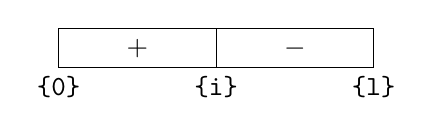
\begin{tikzpicture}
	\draw (0,0) -- (4,0);
    \draw (0,0.5) -- (4,0.5);

    \draw (0,0) -- (0,0.5);
    \draw (0,-0.25) node {\texttt{\string{0\string}}};

    \draw (1,-0.05) node[anchor=south, yshift=0.5mm] {$+$};

    \draw (2,0) -- (2,0.5);
    \draw (2,-0.25) node {\texttt{\string{i\string}}};
    
    \draw (3,0) node[anchor=south] {$-$};
    
    \draw (4,0) -- (4,0.5);
    \draw (4,-0.25) node {\texttt{\string{l\string}}};
\end{tikzpicture}
\end{center}
\caption{A graphical representation of a FunArray.} \label{fig:funarray}

\end{figure}

\noindent The FunArray technique advances the field of abstract interpretation as it is an automatic way to semantically infer segments on arrays. It can easily be introduced to existing analyses without having any significant impact on execution time. It also does not require any additional effort by programmers as it is fully-automatic and it can be combined with any arbitrary abstract domain. In this thesis I will show how I implemented an abstract analyser that utilises the FunArray. I will then test it on a selection of Benchmarks and determine how many of the included assertion obligations can automatically be proven with this approach and how often the analyser at least determines non-trivial invariants for any loops present.



Goal: To implement the FunArray and evaluate it on practical benchmarks

Was kann die Implementierung (Contribution)

Referenzen zu einzelnen Kapiteln (Ich hab so und so viele Invarianten gefunden)

Konkrete Zahlen direkt reinpacken


Array Smashing ist deswegen schlechter, weil die Invarianten mehr als ein

Zeigen dass man nicht-triviale Invarianten hat, aber 


Vielleicht kann man Limitierung DNF umgehen indem man weniger joined und Fallunterscheidungen macht




















 